% !TeX root = ../main.tex

% Edit this title for each week's entry.
\section{Week 2: Multiple Linear Regression (MLR) Models}

\noindent\fbox{\begin{minipage}{\dimexpr\linewidth-2\fboxsep-2\fboxrule}
\textbf{Learning Objectives}
\begin{itemize}
    \item[\textit{Basic}] Write an MLR model in matrix form
    \S\ref{def:mlr}; compute LS estimates via
    $(\mathbf{X}'\mathbf{X})^{-1}\mathbf{X}'\mathbf{Y}$ \S\ref{prop:betahat};
    interpret coefficients, indicators, and interactions
    \S\ref{def:interp}.
    \item[\textit{Adv.}] Derive $\hat{\boldsymbol\beta}$ via matrix
    calculus; encode categorical predictors with dummy variables;
    recognize interaction effects from non-parallel slopes.
\end{itemize}
\end{minipage}}

\subsection{Matrices (Review)}

\begin{definition}[Matrix]
    A rectangular array of elements in $n$ rows and $p$ columns
    (\emph{dimension}/\emph{size} $n\times p$): $n$ = number of rows (1
    per \emph{observation}), $p$ = number of columns (1 per
    \emph{explanatory variable}). \aside{This is exactly \emph{tidy
    data} format: 1 row per observation, 1 column per variable.}
    \[\mathbf{A} = (a_{ij})_{i=1,\dots,n;\,j=1,\dots,p}
    = \begin{pmatrix} a_{11} & \cdots & a_{1p} \\ \vdots & \ddots & \vdots \\ a_{n1} & \cdots & a_{np} \end{pmatrix}\]
    \textbf{Square}: $n=p$. \textbf{Column vector}: $p=1$.
    \textbf{Row vector}: $n=1$.
\end{definition}

\begin{definition}[Transpose, Symmetric]
    If $\mathbf{A}$ is $n\times p$, its \textbf{transpose} $\mathbf{A}'$
    (or $\mathbf{A}^T$) is $p\times n$ (rows $\leftrightarrow$
    columns). $\mathbf{A}$ is \textbf{symmetric} if $\mathbf{A}=\mathbf{A}'$
    (only possible if square).
\end{definition}

\begin{example}[Design Matrix and $\mathbf{X}'\mathbf{X}$]
    \[\mathbf{Y} = \begin{pmatrix}y_1\\y_2\\y_3\end{pmatrix}
    \aside{\text{vector of responses}}, \qquad
    \mathbf{X} = \begin{pmatrix}1 & x_1\\1 & x_2\\1 & x_3\end{pmatrix}
    \aside{\text{always a column of 1's}}\]
    \[\mathbf{X}'\mathbf{X} = \begin{pmatrix}1&1&1\\x_1&x_2&x_3\end{pmatrix}\begin{pmatrix}1 & x_1\\1 & x_2\\1 & x_3\end{pmatrix}
    = \begin{pmatrix}3 & \sum x_i \\ \sum x_i & \sum x_i^2\end{pmatrix}\]
    $\mathbf{X}'\mathbf{X}$ is always square and symmetric.
\end{example}

\subsection{The MLR Model}\label{def:mlr}

\begin{definition}[Simple vs.\ Multiple Regression]
    $p=1$: \textbf{Simple} Regression. $p>1$: \textbf{Multiple}
    Regression, $f:\mathbb{R}^p\to\mathbb{R}$ --- the more general form
    (SLR is MLR with $p=1$).
\end{definition}

\begin{center}
    \begin{minipage}{0.42\linewidth}\centering
        \begin{tikzpicture}[scale=0.9]
            \draw[->] (0,0) -- (3.2,0) node[right] {$X$};
            \draw[->] (0,0) -- (0,2.6) node[above] {$Y$};
            \foreach \x/\y in {0.4/0.5, 0.9/1.3, 1.3/0.9, 1.8/1.7, 2.2/1.5, 2.6/2.1}{
                \fill (\x,\y) circle (1.3pt);
            }
            \draw[thick,blue!60!black] (0.1,0.3) -- (2.9,2.2);
        \end{tikzpicture}
        \\[2pt] \textit{\small 1 predictor: line of best fit}
    \end{minipage}
    \hfill
    \begin{minipage}{0.52\linewidth}\centering
        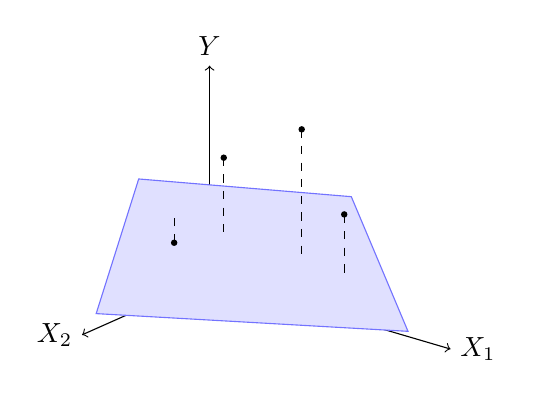
\begin{tikzpicture}[scale=0.9]
            \draw[->] (0,0) -- (0,3.0) node[above] {$Y$};
            \draw[->] (0,0) -- (3.4,-1.0) node[right] {$X_1$};
            \draw[->] (0,0) -- (-1.8,-0.8) node[left] {$X_2$};
            \filldraw[fill=blue!12,draw=blue!55] (-1.6,-0.5) -- (2.8,-0.75) -- (2.0,1.15) -- (-1.0,1.4) -- cycle;
            \foreach \x/\y/\z in {0.2/1.7/0.55, 1.3/2.1/0.25, -0.5/0.5/0.9, 1.9/0.9/0.05}{
                \fill (\x,\y) circle (1.3pt);
                \draw[dashed] (\x,\y) -- (\x,\z);
            }
        \end{tikzpicture}
        \\[2pt] \textit{\small 2 predictors: plane in $\mathbb{R}^3$}
    \end{minipage}
    \\[4pt] \textit{\small $p>2$ predictors: hyperplane in $\mathbb{R}^{p+1}$ (can't visualize directly)}
\end{center}

\begin{definition}[MLR Model]
    For individual $i=1,\dots,n$:
    \[Y_i = \beta_0+\beta_1x_{i1}+\cdots+\beta_px_{ip}+\epsilon_i
    = \mathbf{x}_i'\boldsymbol\beta+\epsilon_i, \qquad \epsilon_i\overset{iid}\sim N(0,\sigma^2)\]
    where $\mathbf{x}_i'=(1,x_{i1},\dots,x_{ip})$ is treated as
    fixed/known. Stacking over $i$: $\boxed{\mathbf{Y}=\mathbf{X}\boldsymbol\beta+\boldsymbol\epsilon}$,
    \[\mathbf{X} = \begin{pmatrix}\mathbf{x}_1'\\\vdots\\\mathbf{x}_n'\end{pmatrix}
    = \begin{pmatrix}1&x_{11}&\cdots&x_{1p}\\\vdots&\vdots&\ddots&\vdots\\1&x_{n1}&\cdots&x_{np}\end{pmatrix},
    \quad \boldsymbol\beta=\begin{pmatrix}\beta_0\\\vdots\\\beta_p\end{pmatrix},
    \quad \boldsymbol\epsilon=\begin{pmatrix}\epsilon_1\\\vdots\\\epsilon_n\end{pmatrix}
    \sim N(\mathbf{0}_n,\sigma^2\mathbf{I}_n)\]
    \aside{$\sigma^2\mathbf{I}_n$: multivariate normal, diagonal covariance
    $\mathrm{diag}(\sigma^2,\dots,\sigma^2)$ --- same $\sigma^2$, i.i.d.\
    as in SLR.} $E[Y\mid\mathbf{X}=\mathbf{x}]=\beta_0+\beta_1x_1+\cdots+\beta_px_p$,
    $\Var[Y\mid\mathbf{X}=\mathbf{x}]=\sigma^2$ (again abbreviated
    $E[Y],\Var[Y]$, always conditioning on $\mathbf{X}$).
\end{definition}

\aside{$\mathbf{x}$ is $(p+1)$-dimensional: 1 intercept $+$ $p$
predictors. (Some sources instead say $p$ entries total, $p-1$
predictors --- check convention.)}

\begin{remark}[Design Matrix Conventions]
    \begin{itemize}
        \item First column is \textbf{always} 1's (intercept).
        \item Must be numeric --- categorical predictors need
        \textbf{indicator (dummy) variables}, a.k.a.\ \emph{one-hot encoding}.
        \item Each observation must fall in exactly 1 category.
    \end{itemize}
\end{remark}

\begin{example}[Encoding a Categorical Predictor]
    \textbf{2 levels} (e.g.\ transmission, automatic/manual): 1
    indicator suffices, $X=\mathbb{I}(\text{manual})$.
    \\ \textbf{$c$ levels} (e.g.\ colour Blue/Red/Yellow): pick 1
    \textbf{baseline} (in R: first level alphanumerically), need
    $c-1$ indicators. $X_2=\mathbb{I}(\text{Red})$, $X_3=\mathbb{I}(\text{Yellow})$;
    both 0 $\Rightarrow$ Blue.
\end{example}

\begin{example}[Dimension of $\mathbf{X}$]\label{ex:dim}
    7 numeric predictors, $n=45$: $\mathbf{X}$ is $45\times8$ (1
    intercept $+$ 7 predictors). \\ 1 continuous predictor $+$ 1
    categorical predictor with 10 levels, $n=100$: $\mathbf{X}$ is
    $100\times11$ (1 intercept $+$ 1 continuous $+$ 9 dummy columns).
    \aside{Want $p$ small relative to $n$ --- helps ensure
    $\mathbf{X}'\mathbf{X}$ is invertible.}
\end{example}

\aside{Discrete predictor taking values $1$--$100$: continuous or
categorical? Ask: can the levels be ordered? Is the difference between
adjacent levels always the same (e.g.\ $2-1\overset{?}{=}100-99$)? If
yes to both, treat as continuous.}

\subsection{Estimation via Least Squares}

\begin{definition}[Residual Sum of Squares]
    \[RSS(\hat{\boldsymbol\beta}) = \sum_{i=1}^n\hat\epsilon_i^2
    = \sum_{i=1}^n\big(Y_i-\mathbf{x}_i'\hat{\boldsymbol\beta}\big)^2
    = (\mathbf{Y}-\mathbf{X}\hat{\boldsymbol\beta})'(\mathbf{Y}-\mathbf{X}\hat{\boldsymbol\beta})
    = (\mathbf{Y}-\hat{\mathbf{Y}})'(\mathbf{Y}-\hat{\mathbf{Y}})\]
    Same LS procedure as SLR: (1) set up the estimating equation, (2)
    differentiate w.r.t.\ $\boldsymbol\beta$ and set to $\mathbf{0}$,
    (3) solve for $\hat{\boldsymbol\beta}$, (4) unique minimizer iff
    $\mathbf{X}'\mathbf{X}$ is invertible (\emph{full rank}) --- see
    \emph{multicollinearity}.
\end{definition}

\aside{Matrix calculus (Rencher \& Schaalje \S2.14): for constants
$\mathbf{a}$, $\partial(\mathbf{a}'\mathbf{x})/\partial\mathbf{x}=\mathbf{a}$;
for symmetric $\mathbf{A}$, $\partial(\mathbf{x}'\mathbf{A}\mathbf{x})/\partial\mathbf{x}=2\mathbf{A}\mathbf{x}$;
and $(\mathbf{A}\mathbf{B})'=\mathbf{B}'\mathbf{A}'$.}

\begin{proposition}[LS Estimator]\label{prop:betahat}
    Assuming $(\mathbf{X}'\mathbf{X})^{-1}$ exists,
    \[\boxed{\hat{\boldsymbol\beta} = (\mathbf{X}'\mathbf{X})^{-1}\mathbf{X}'\mathbf{Y}}\]
    In practice, component matrices are easy to build from sums; only
    the inverse needs software.
    \[\mathbf{X}'\mathbf{X} = \begin{pmatrix}
    n & \sum x_{i1} & \cdots & \sum x_{ip}\\
    \sum x_{i1} & \sum x_{i1}^2 & \cdots & \sum x_{i1}x_{ip}\\
    \vdots & \vdots & \ddots & \vdots\\
    \sum x_{ip} & \sum x_{i1}x_{ip} & \cdots & \sum x_{ip}^2
    \end{pmatrix}, \qquad
    \mathbf{X}'\mathbf{Y} = \begin{pmatrix}\sum y_i\\\sum x_{i1}y_i\\\vdots\\\sum x_{ip}y_i\end{pmatrix}\]
\end{proposition}

\begin{definition}[Hat Matrix]
    $\hat{\mathbf{Y}}=\mathbf{X}\hat{\boldsymbol\beta}=\mathbf{X}(\mathbf{X}'\mathbf{X})^{-1}\mathbf{X}'\mathbf{Y}=\mathbf{H}\mathbf{Y}$,
    where $\mathbf{H}=\mathbf{X}(\mathbf{X}'\mathbf{X})^{-1}\mathbf{X}'$ is
    the \textbf{hat}/\textbf{projection}/\textbf{influence} matrix:
    \emph{idempotent} ($\mathbf{H}^2=\mathbf{H}$), and projects $\mathbf{Y}$
    onto $\hat{\mathbf{Y}}$ (\emph{model space}).
    \begin{itemize}
        \item Diagonal entries $h_{ii}=\mathbf{x}_i'(\mathbf{X}'\mathbf{X})^{-1}\mathbf{x}_i$
        are \textbf{leverages}: high leverage $\Rightarrow$ \emph{outlier} in
        $X$, potential high influence on $\hat{\boldsymbol\beta}$ if
        deleted.
        \item Residuals: $\hat{\boldsymbol\epsilon}=\mathbf{Y}-\hat{\mathbf{Y}}=(\mathbf{I}_n-\mathbf{H})\mathbf{Y}=\mathbf{M}\mathbf{Y}$,
        where $\mathbf{M}=\mathbf{I}_n-\mathbf{H}$ is the \textbf{residual
        maker} ($\hat{\boldsymbol\epsilon}=\mathbf{M}\mathbf{Y}$) or
        \textbf{annihilator} matrix ($\mathbf{M}\mathbf{X}=\mathbf{0}$).
    \end{itemize}
\end{definition}

\begin{center}
    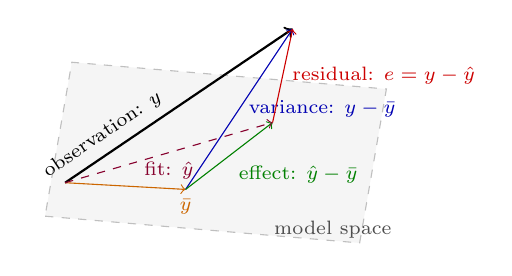
\begin{tikzpicture}[scale=0.85]
        \coordinate (O) at (0,0);
        \coordinate (Ybar) at (1.8,-0.1);
        \coordinate (Yhat) at (3.1,0.9);
        \coordinate (Y) at (3.4,2.3);
        \filldraw[fill=gray!8,draw=gray!50,dashed] (-0.3,-0.5) -- (4.4,-0.9) -- (4.8,1.4) -- (0.1,1.8) -- cycle;
        \node[gray!60!black] at (4.0,-0.7) {\scriptsize model space};
        \draw[->,thick] (O) -- (Y) node[midway, above left, sloped] {\scriptsize observation: $y$};
        \draw[->,orange!80!black] (O) -- (Ybar) node[below] {\scriptsize $\bar y$};
        \draw[->,blue!70!black] (Ybar) -- (Y) node[midway,right] {\scriptsize variance: $y-\bar y$};
        \draw[->,green!50!black] (Ybar) -- (Yhat) node[midway,below right] {\scriptsize effect: $\hat y - \bar y$};
        \draw[->,dashed,purple!70!black] (O) -- (Yhat) node[midway,below] {\scriptsize fit: $\hat y$};
        \draw[->,red!80!black] (Yhat) -- (Y) node[midway,right] {\scriptsize residual: $e=y-\hat y$};
    \end{tikzpicture}
    \\[2pt] \textit{\small $\hat y$ is the orthogonal projection of $y$ onto the model space; $e\perp$ model space.}
\end{center}

\subsection{Application Example}

\begin{example}[\texttt{mtcars} Dataset]\label{ex:mtcars}
    32 automobiles (1973--74 models); using \texttt{mpg} (response),
    \texttt{disp}, \texttt{hp}, \texttt{wt} (predictors):
    \[mpg_i = \beta_0+\beta_1disp_i+\beta_2hp_i+\beta_3wt_i+\epsilon_i\]
    Fitted: $\widehat{mpg}=37-0.009\,disp-0.03\,hp-3.8\,wt$.
    \aside{\texttt{disp} not significant ($p=0.93$); \texttt{hp}, \texttt{wt}
    significant ($p=0.011$, $0.001$); $R^2=0.827$.}
\end{example}

\begin{example}[Rencher \& Schaalje Ex.\ 7.2 --- Worked by Hand]\label{ex:rencher}
    12 observations of $Y$ on $X_1,X_2$ give
    $\sum y_i=90$, $\sum x_{i1}=52$, $\sum x_{i2}=102$,
    $\sum x_{i1}^2=296$, $\sum x_{i2}^2=1004$, $\sum x_{i1}x_{i2}=536$,
    $\sum x_{i1}y_i=482$, $\sum x_{i2}y_i=872$, so
    \[\mathbf{X}'\mathbf{X}=\begin{pmatrix}12&52&102\\52&296&536\\102&536&1004\end{pmatrix},
    \qquad \mathbf{X}'\mathbf{Y}=\begin{pmatrix}90\\482\\872\end{pmatrix}\]
    Inverting (software) and multiplying:
    \[\hat{\boldsymbol\beta}=(\mathbf{X}'\mathbf{X})^{-1}\mathbf{X}'\mathbf{Y}
    \approx\begin{pmatrix}5.375\\3.012\\-1.285\end{pmatrix}
    \ \Rightarrow\ \hat y_i = 5.375+3.012x_{i1}-1.285x_{i2}\]
\end{example}

\begin{example}[Prediction]
    Using Ex.\ \ref{ex:rencher} at $X_1=5$, $X_2=9$:
    \[\hat y = 5.375+3.012(5)-1.285(9) = 8.87\]
    Interpretation: the mean response when $X_1=5,X_2=9$ is $8.87$.
\end{example}

\subsection{Interpreting Coefficients}\label{def:interp}

\begin{definition}[Coefficient Interpretation]
    $\hat Y=\hat E[Y\mid\mathbf{X}=\mathbf{x}]=\hat\beta_0+\hat\beta_1x_1+\cdots+\hat\beta_px_p=\mathbf{x}'\hat{\boldsymbol\beta}$.
    \begin{itemize}
        \item $\hat\beta_0$: estimated avg.\ $Y$ when \emph{all}
        predictors are 0.
        \item $\hat\beta_j$ ($j\geq1$): estimated avg.\ change in $Y$
        per 1-unit increase in $x_j$, \textbf{holding all other
        predictors fixed}.
    \end{itemize}
\end{definition}

\begin{remark}[Conditional Nature of MLR]
    Coefficients are only valid \emph{holding other predictors fixed}
    --- an SLR fit on one predictor alone can differ drastically
    (even in sign) from its MLR coefficient. In Ex.\ \ref{ex:rencher},
    SLR gives $\hat y=1.86+1.30x_1$ and $\hat y=0.86+0.78x_2$ (both
    \emph{positive} slopes), but jointly $\hat\beta_2=-1.285$
    (\emph{negative}) --- because MLR's $\hat\beta_2$ is the effect of
    $X_2$ \emph{within} a fixed value of $X_1$ (a \emph{partial
    regression}), not \emph{marginally}. \aside{Ignoring a correlated
    predictor can flip the apparent sign of an effect.}
\end{remark}

\begin{center}
    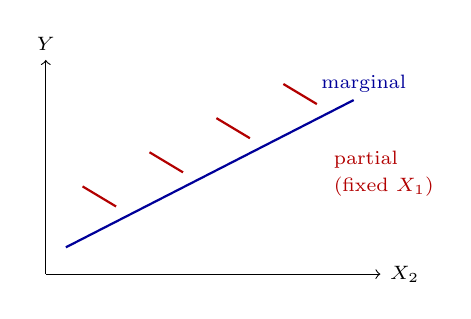
\begin{tikzpicture}[scale=0.85]
        \draw[->] (0,0) -- (5,0) node[right] {\scriptsize $X_2$};
        \draw[->] (0,0) -- (0,3.2) node[above] {\scriptsize $Y$};
        \draw[thick,blue!60!black] (0.3,0.4) -- (4.6,2.6);
        \node[blue!60!black] at (4.75,2.85) {\scriptsize marginal};
        \draw[thick,red!70!black] (0.55,1.31) -- (1.05,1.01);
        \draw[thick,red!70!black] (1.55,1.82) -- (2.05,1.52);
        \draw[thick,red!70!black] (2.55,2.33) -- (3.05,2.03);
        \draw[thick,red!70!black] (3.55,2.84) -- (4.05,2.54);
        \node[red!70!black,align=left] at (5.05,1.5) {\scriptsize partial\\[-2pt]\scriptsize (fixed $X_1$)};
    \end{tikzpicture}
    \\[2pt] \textit{\small Marginal slope (blue, ignoring $X_1$) vs.\ partial slopes (red, at fixed $X_1$) --- opposite sign here.}
\end{center}

\begin{example}[Interpreting an Indicator Variable]
    Add \texttt{am} ($\mathbb{I}(am=1)=$ manual) to the \texttt{mtcars}
    model:
    \[\widehat{mpg}=\hat\beta_0+\hat\beta_1disp+\hat\beta_2hp+\hat\beta_3wt+\hat\beta_4\,\mathbb{I}(am=1),
    \qquad \hat\beta_4=2.16\]
    $\hat\beta_4$ = estimated avg.\ difference in $mpg$ between manual
    and automatic transmission, holding \texttt{disp}, \texttt{hp},
    \texttt{wt} fixed: the intercept is $\hat\beta_0$ when $am=0$, and
    $\hat\beta_0+\hat\beta_4$ when $am=1$ --- a parallel vertical shift,
    same slopes.
\end{example}

\begin{definition}[Interaction]\label{def:interaction}
    An \textbf{interaction effect} exists when the joint effect of two
    (or more) predictors differs from their separate effects; include
    it as a product term $x_jx_k$ (works for any combination of
    numeric/categorical predictors). \aside{E.g.\ is the
    smoking--lung-cancer association the same in rural vs.\ urban
    areas? Does a renovation raise price in the suburbs but not
    downtown? Does drug dosage increase response in females but
    decrease it in males?}
\end{definition}

\aside{``Linear'' still just means linear in $\boldsymbol\beta$: e.g.\
$Y=\beta_0+\beta_1x_1x_2+\beta_2\sin(x_2)+\beta_3x_3^2$ is a linear
model.}

\begin{example}[Interaction --- \texttt{mtcars}]
    \[\widehat{mpg}=\hat\beta_0+\hat\beta_1wt+\hat\beta_2\mathbb{I}(am=1)+\hat\beta_3\big(wt\times\mathbb{I}(am=1)\big)\]
    Fitted: $31.42-3.79wt+14.88\,\mathbb{I}(am=1)-5.30\big(wt\times\mathbb{I}(am=1)\big)$.
    Slope of \texttt{wt} is $-3.79$ for automatic ($am=0$); for manual
    ($am=1$) it is $5.30$ \emph{more negative}, i.e.\ $-9.09$ ---
    different intercept \emph{and} slope per group.
\end{example}

\begin{remark}[Detecting Interaction Visually]
    No interaction $\Rightarrow$ fitted lines/planes for each category
    are \textbf{parallel}. \textbf{Non-parallel} slopes (e.g.\ \texttt{mpg} vs.\
    \texttt{wt} across \texttt{cyl} $\in\{4,6,8\}$) suggest an
    interaction (formal test later). With $>2$ predictors, ``lines''
    become planes/hyperplanes.
\end{remark}

\aside{Plotting caution: don't lead the viewer by extrapolating fitted
lines beyond each group's observed range --- and don't recode a numeric
predictor (e.g.\ \texttt{cyl}) as categorical for a plot like this
unless there's a substantive reason to.}

\begin{center}
    \begin{minipage}{0.46\linewidth}\centering
        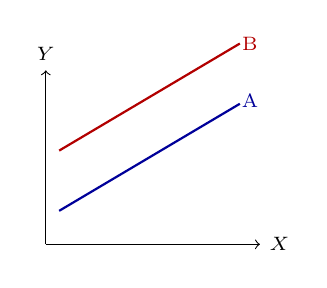
\begin{tikzpicture}[scale=0.85]
            \draw[->] (0,0) -- (3.2,0) node[right] {\scriptsize $X$};
            \draw[->] (0,0) -- (0,2.6) node[above] {\scriptsize $Y$};
            \draw[thick,blue!60!black] (0.2,0.5) -- (2.9,2.1);
            \draw[thick,red!70!black] (0.2,1.4) -- (2.9,3.0);
            \node[blue!60!black] at (3.05,2.15) {\scriptsize A};
            \node[red!70!black] at (3.05,3.0) {\scriptsize B};
        \end{tikzpicture}
        \\[2pt] \textit{\small No interaction: parallel slopes}
    \end{minipage}
    \hfill
    \begin{minipage}{0.46\linewidth}\centering
        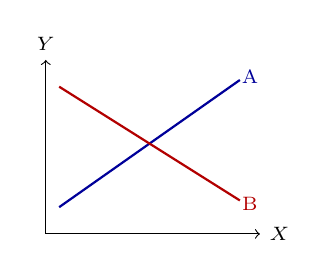
\begin{tikzpicture}[scale=0.85]
            \draw[->] (0,0) -- (3.2,0) node[right] {\scriptsize $X$};
            \draw[->] (0,0) -- (0,2.6) node[above] {\scriptsize $Y$};
            \draw[thick,blue!60!black] (0.2,0.4) -- (2.9,2.3);
            \draw[thick,red!70!black] (0.2,2.2) -- (2.9,0.5);
            \node[blue!60!black] at (3.05,2.35) {\scriptsize A};
            \node[red!70!black] at (3.05,0.45) {\scriptsize B};
        \end{tikzpicture}
        \\[2pt] \textit{\small Interaction: non-parallel (crossing) slopes}
    \end{minipage}
\end{center}

\aside{A categorical predictor with $c>2$ levels still only needs
$c-1$ dummy columns, generated automatically by software (e.g.\
\texttt{factor(cyl)} for \texttt{cyl}$\in\{4,6,8\}$ creates 2 columns,
baseline = smallest level, 4).}

\begin{example}[Try at Home]
    Given the data below:
    \begin{center}
    \begin{tabular}{ccc}
        \toprule
        $Y$ & $X_1$ & $X_2$ \\
        \midrule
        $-0.2$ & $0.5$ & $0.5$ \\
        $-1.1$ & $0.8$ & $0.7$ \\
        $-0.8$ & $0.6$ & $-0.5$ \\
        $-0.7$ & $-0.2$ & $-0.5$ \\
        \bottomrule
    \end{tabular}
    \end{center}
    Write out $\mathbf{X}$ (with intercept column) and compute
    $\hat{\boldsymbol\beta}=(\mathbf{X}'\mathbf{X})^{-1}\mathbf{X}'\mathbf{Y}$
    by hand; check against \texttt{lm()}.
\end{example}
